\documentclass[12pt]{article}
\usepackage[margin=1in]{geometry}
\usepackage{amsmath, amssymb}
\usepackage{tabularx}
\usepackage{array}
\usepackage{booktabs}
\usepackage{graphicx}
\usepackage{pdflscape}
\usepackage{caption}
\usepackage{hyperref}
\usepackage{float}
\hypersetup{colorlinks=true, linkcolor=blue, urlcolor=blue}
\usepackage{longtable}
\captionsetup{font=small}
\usepackage[table,xcdraw]{xcolor}
\usepackage{titlesec}
\usepackage{threeparttable}
\usepackage[utf8]{inputenc}
\usepackage[backend=biber,style=apa]{biblatex}
\addbibresource{references.bib}

% ====== FONT ======

\titleformat{\section}
  {\normalfont\normalsize\bfseries}{\thesection}{1em}{}

\titleformat{\subsection}
  {\normalfont\normalsize\bfseries}{\thesubsection}{1em}{}

\titleformat{\subsubsection}
  {\normalfont\normalsize\bfseries}{\thesubsubsection}{1em}{}


% ====== PAGE GEOMETRY ======
\geometry{
  left=1in, right=1in,
  top=1in, bottom=1in
}

% ====== COLORS ======
\definecolor{gray6}{RGB}{242,242,242}

% ====== CAPTION STYLE ======
\captionsetup[longtable]{labelfont=bf, font=small, 
  singlelinecheck=false, 
  skip=0pt}

\title{Interdependence Composition, Conflict, and Cooperation}
\author{Nazim Uras Demir \footnote{Nazim Uras Demir is a Visiting Assistant Professor at Loyola Marymount University (\texttt{xxx})}
 }
\date{July 2025}

\begin{document}
\maketitle

\begin{abstract}
This is your abstract. 
\end{abstract}

\newpage  % Start new page after abstract

\section{Introduction}
How does trade composition influence cooperation between states? In 2022, Japan's Diet approved the Economic Security Promotion Act \parencite{japanESPA2022}--a comprehensive bill to hedge the country's economy against growing geoeconomic instability. One of the four pillars of the bill addresses diversification of supply chains to access goods defined as specific critical materials that are necessary for Japan's national security. On the other side of the Pacific, the US enacted the CHIPS and Science Act \parencite{uscongresschips2022} and the Inflation Reduction Act \parencite{uscongressira2022}, both with specific clauses to address securing access to and production of goods deemed ``strategic". Across the Pond, the EU Parliament unveiled its Economic Security Strategy \parencite{eu2023economicsecurity}, discussing the importance of access to ``critical" products. Beyond policy circles, curiosity about ``strategic goods" has been on the rise also: Google Trends suggests a gradual increase in the number of queries that were virtually zero two decades ago. Trade interdependence is no longer treated as a monolith; attention is turning to the composition of goods that shape its structure.

Despite extensive legislation, the concept of the ``strategic good" remains anchored on apparent dual-use products \parencite{schelling2008arms}, and several others, often identified through heuristics related to technological or economic importance. The same handful of commodities—semiconductors, critical minerals, lithium-ion batteries, medical products—are repeatedly cited in economic security legislation. Yet many other goods, particularly intermediate inputs that flow through global supply chains, are equally critical but often overlooked. While scholars of international relations have produced insights into how such goods shape national security and interstate relations \parencites{drezner2021uses,ding2021logic,kim2024us, lee2024us, vekasi2021geoeconomics, gholz2021market, beaumier2024cross}, what is ``strategic" remains controversial as \textcite{baldwin2020statecraft} notes.

The strategic value of a good is defined only in relation to a broader universe of non-strategic goods: identification of what \textit{is} strategic necessitates identification of what \textit{is not}. This requires a framework that clearly delineates and mutually excludes different categories of goods. Additionally, the strategic value of a commodity is never fixed; it evolves with technological change. Timber, once vital to the naval power of Greek, Roman, and British fleets, gradually ceded its strategic importance to steel and, later, to modern advanced metal alloys. In this paper, I introduce a framework that addresses this gap by systematically evaluating the relative value of all commodities over time and mapping the compositional anatomy of each country’s exports.

Understanding the composition of trade is important in studying economic interdependence, peace, and conflict—especially amid rising legislation focused on economic security. Although economic interdependence continues to shape international politics \parencite{keohane2020globalization, solingen2025global}, its outcomes remain elusive \parencites{brooks2024trade, chang2017economic}. While the subject has remained contentious since the time of Thucydides, contemporary research—building on \textcite{hirschman1980}—has shown that interdependence can foster peace \parencite{russett1998third}, fuel conflict \parencite{barbieri1996economic}, or produce outcomes conditioned by expectations \parencite{copeland2014}, democracy \parencite{gelpi2008}, nationalism \parencite{choi2023does}, great power status \parencite{levy2023systemic}, capitalism \parencite{gartzke2007}, institutions \parencite{petersonwen2021}, and regime-specific survival dynamics \parencite{solingen2021}, among others. While many studies highlight the pacifying effects of trade—\textit{doux commerce}, as Montesquieu called it, or \textit{Handelsgeist}, in Kant’s writings—trade is increasingly being securitized and weaponized. Yet we still know little about how the compositional structure of exports shapes patterns of conflict and cooperation between states.

I have two research objectives. First, I introduce a framework for identifying the relative importance of all commodities in the global marketplace over time, using universal attributes that apply to all of them. This framework opens the black box of trade flows and defines the compositional dimensions of interdependence—bridging the gap between micro-level analyses that focus on narrow sets of goods and macro-level studies that rely on aggregate trade flows. It also allows researchers to characterize the composition of a country’s exports to its trade partners. In specific, using granular commodity-level data (HS6) from the UN Comtrade Database, I construct three core attributes of each product: centrality (its global economic importance), exclusivity (its market concentration), and complexity (its technological sophistication, based on the Economic Complexity Index). These attributes are then used to generate three key measures of export composition: distance from the global trade centroid, entropy across product types, and a theory-weighted composite score.

Second, I examine how the compositional structure of exports relates to patterns of interstate conflict and cooperation. Most studies of interdependence mentioned above rely on macro-level analyses using aggregate trade data. Some, however, examine interdependence at the commodity level—though often through micro-analyses limited to a narrow subset of goods. Among those that use granular trade data, for example, \textcite{reuveny1998bilateral}, \textcite{dorussen2006heterogeneous}, \textcite{goenner2010toys}, and \textcite{zeng2024microchips} explore heterogeneity within exports focusing on strategic goods, while in a more expansive setting, \textcite{chatagnier2017} examines portfolio similarity between trade partners, \textcite{peterson2016} explore intra-industry flows using disaggregated data, and \textcite{kim2020measuring} identify clusters of countries based on trade profiles. To the best of my knowledge, no existing study has tested hypotheses linking export composition, defined through multiple commodity attributes using granular data, to political outcomes. Here, using a panel of 170,598 directed dyad-years spanning 2000 to 2020, I estimate the relationship between compositional structure of exports and political interaction intensity, drawing on event-level data from the Integrated Crisis Early Warning System (ICEWS). I estimate outcomes across four event domains—all interactions combined, as well as diplomatic, armed, and economic interactions separately. For each domain, I assess the association with export composition based on the full set of events, as well as separately for cooperation-only and conflict-only events.

%Findings as contributions

The next section reviews the literature on economic interdependence and international security. Section three specifies empirical expectations about the association between interdependence composition and interstate interactions. Section four introduces the research design and presents the results of the empirical analysis. Section five explores the alignment between the results and the expectations. Section six discusses implications and concludes by offering routes for future research. 

\section{Trade Interdependence and Security}
Trade interdependence refers to a relationship in which the economic decisions of one state have consequential effects on another, and vice versa \parencites{hirschman1980, keohane2012power}. Its effects on security is a contentious debate among scholars of international relations, with some suggesting that it leads to peace \parencites{}

is at the core of the growing scholarship on economic statecraft \parencite{aggarwal2025oxford, blackwill2016war, chen2023wars, ferguson2025states, katada2022east}

\section{Empirical Expectations}
\section{Research Design}
This section introduces a systematic approach to quantify the structural composition of trade dependencies between states. These composition measures are designed to complement the flow measures--salience and symmetry--often used in trade interdependence analysis. I begin by evaluating individual traded commodities (HS6) along three dimensions discussed above: economic \textit{centrality}, \textit{exclusivity}, and \textit{complexity}. These commodity-level compositional attributes are then aggregated into directed dyadic measures.

\subsection{Commodity Attributes}
Each HS6-level commodity is evaluated on three standardized dimensions that capture its role in structuring interdependence:

\subsection*{\textit{Centrality} ($C$)}
Centrality is measured as the commodity's share of total global trade in a given year: 
\begin{equation}
C_i = \frac{\text{Trade Value}_i}{\sum_{j} \text{Trade Value}_j}
\end{equation}

\subsection*{\textit{Exclusivity} ($E$)}

Exclusivity is based on the Herfindahl-Hirschman Index (HHI) of global export market concentration:\footnote{See \textcite{goenner2010toys}, \textcite{arriola2024}, \textcite{chimits2024} for similar applications.}
\begin{equation}
\text{HHI}_i = \sum_{e \in E_i} s_{ie}^2 \quad \text{where } s_{ie} = \frac{\text{Exports}_{ie}}{\sum_{e} \text{Exports}_{ie}}, \quad \text{and } s_{ie} \geq 2.5\%
\end{equation}

I incldue only exporters with at least 2.5\% market share to avoid inflating exclusivity due to minor senders. \footnote{For example, there were 161 countries with exports of memory integrated circuits (HS854232) in 2023 according to UN Comtrade data. Among these, only six--South Korea, China, Taiwan, Singapore, Japan, and Malaysia--had a share higher than 2.5\%.} The inverse of HHI (after log-transform) is used to reflect availability across suppliers.
  
\subsection*{\textit{Complexity} ($K$)}
Complexity is proxied by Economic Complexity Index (ECI) of \textcite{hausmann2014atlas}, $K_i = \text{ECI}_i$. It reflects the technological sophistication of a product.

I then rank-transform and standardize all three attributes:
\begin{equation}
C_z, \ A_z, \ K_z \in \text{rank}(C_i, A_i, K_i) \xrightarrow{\text{standardize}} \mathcal{N}(0, 1)
\end{equation}

Each commodity is finally classified into one of 8 types based on whether it scores above or below the median on each dimension (High = H, Low = L), forming labels like HHL, LHH, etc.

\vspace{1em}

\begin{table}[H]
\small
\centering
\caption{Selected HS6-Level Commodities and Cubelet Classification (2020)}
\resizebox{\textwidth}{!}{
\begin{tabular}{llrrrccccl}
\toprule
Code & Commodity & $C_z$ & $E_z$ & $K_z$ & High $C$ & High $E$ & High $K$ & Cubelet \\
\midrule
%901210 & Microscopes                    & 0.19  & 0.70  & 1.70  & TRUE  & FALSE  & TRUE  & HLH \\
%854150 & Semiconductors                 & 0.73  & -0.01 & 1.32  & TRUE  & TRUE & TRUE  &  HHH \\
%310230 & Ammonium nitrate               & 0.10  & 0.11  & -1.07 & TRUE  &  FALSE & FALSE & HLL \\
%850710 & Lead-acid accumulators        & 1.42  & -1.52 & -0.47 & TRUE  & TRUE & FALSE & HHL \\
%841780 & Industrial furnaces           & -0.60 & 0.64  & 1.08  & FALSE & FALSE  & TRUE  & LHL \\
%110812 & Maize starch                  & -0.60 & -1.09 & -0.57 & FALSE & TRUE & FALSE &  LLH \\
%853329 & Electrical resistors          & -0.80 & -1.49 & 1.02  & FALSE &  TRUE & TRUE  & LLL \\
%540753 & Polyester woven fabric        & -0.94 & 0.92  & -0.08 & FALSE & FALSE  & FALSE & LHH \\
\bottomrule
\end{tabular}}
\end{table}

The cube plot below shows commodities as dots arranged in a three-dimensional space defined by their rank-standardized values on centrality, exclusivity, and complexity. Each axis slices the commodity landscape into high and low halves, segmenting the space into eight distinct cubelets. Dots represent individual commodities. Clusters of dots in different corners of the cube represent commodity groups that share similar structural positions in the global economy. For example, dense concentrations in the front-right-top corner indicate commodities with high centrality, high exclusivity, and high complexity. \footnote{Color is used to distinguish these cubelets. Interactive 3D cube plots visualizing the full commodity distribution are available in the online appendix.}

\begin{figure}[H]
    \centering
    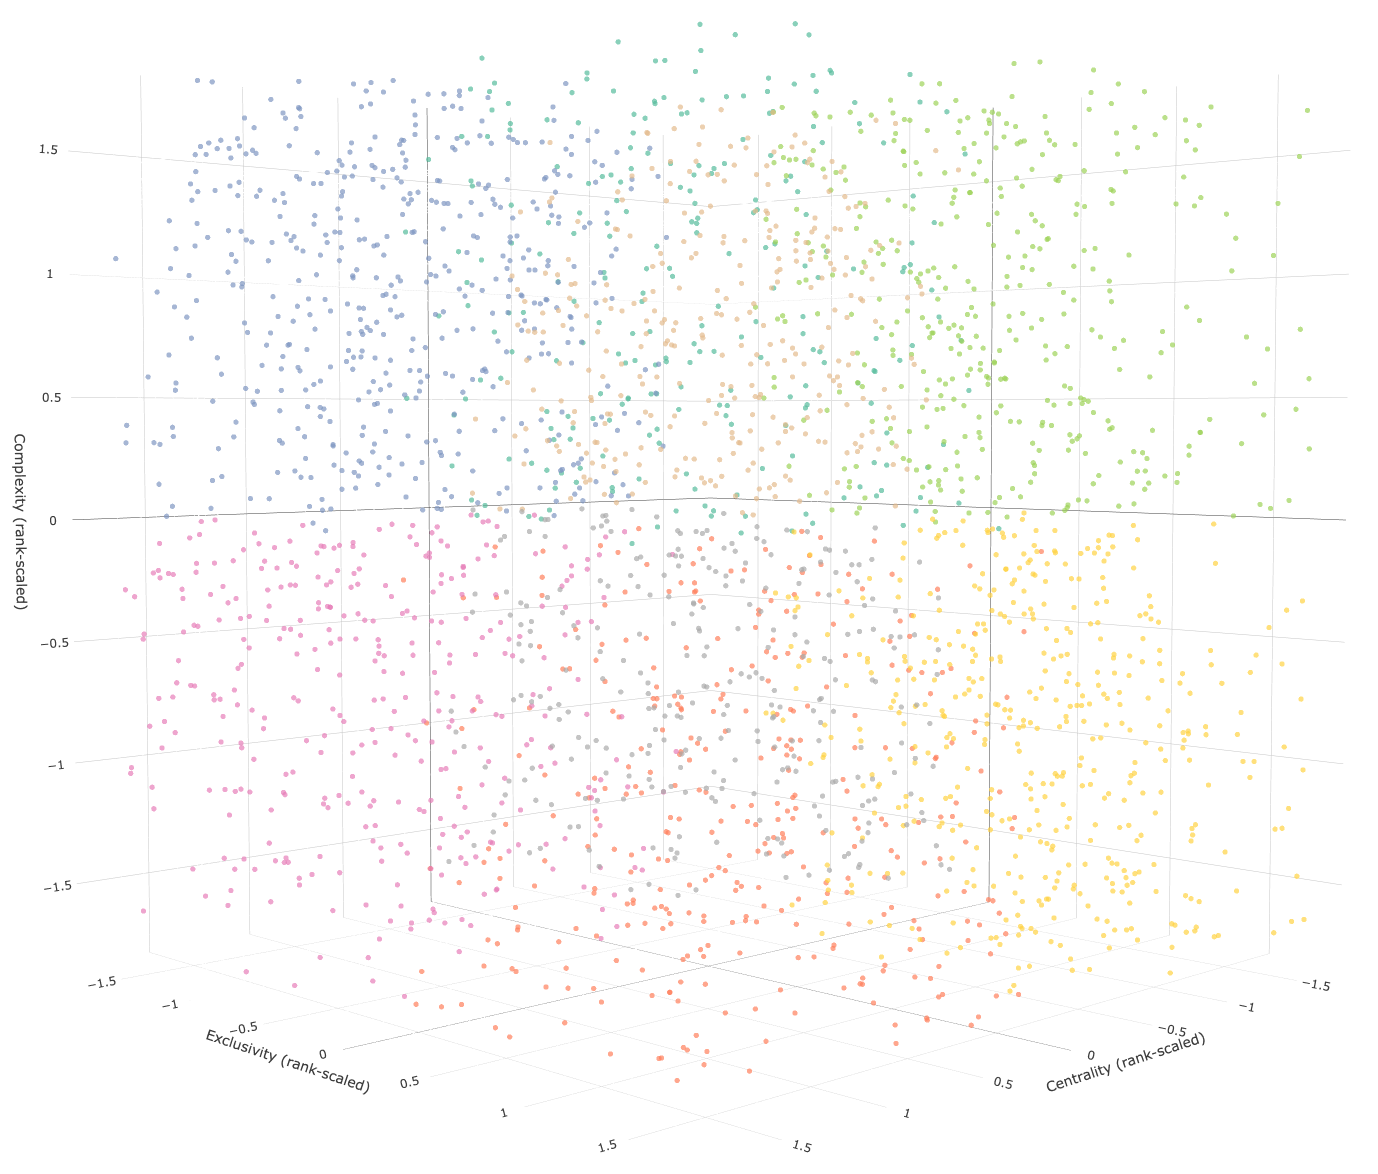
\includegraphics[width=0.85\textwidth]{figures/commodity_cube_plot_2020.png}
    \caption{Classification of Commodities by Centrality, Exclusivity, and Complexity}
    \label{fig:cube_screenshot}
\end{figure}

\subsection{Composition Measures}

Let $i \rightarrow j$ denote a directed dyad of trade from exporter $i$ to importer $j$. I compute four indicators to characterize the structure and strategic intensity of bilateral export bundles.

\subsection*{\textit{Distance from Origin}}

I summarize the trade flow’s average structural features by weighting each commodity’s attribute score ($x_k$) by its trade value:

\begin{equation}
\text{Mean}_x^{(ij)} = \frac{ \sum_{k} \text{Trade}_{k}^{(ij)} \cdot x_k }{ \sum_{k} \text{Trade}_{k}^{(ij)} }
\end{equation}

Where $x_k \in \{C_z, E_z, K_z\}$, representing standardized scores for centrality, exclusivity, and complexity respectively. Next, I use this measure to capture the strategic intensity of a trade flow by computing the Euclidean distance from the origin in the 3D attribute space:

\begin{equation}
D_{ij} = \sqrt{ \left( \text{Mean}_{C}^{(ij)} \right)^2 + \left( \text{Mean}_{E}^{(ij)} \right)^2 + \left( \text{Mean}_{K}^{(ij)} \right)^2 }
\end{equation}

Higher values indicate bundles with more central, difficult to access, and complex commodities relative to lower values.

\subsection*{\textit{Entropy Value}}

Each commodity $k$ exported from country $i$ to $j$ is assigned to one of eight cubelet types based on whether the $k$'s standardized attribute scores exceed the global median:

\begin{align*}
\texttt{H} &\quad \text{if } x_k \geq \text{median}(x), \\
\texttt{L} &\quad \text{otherwise}, \quad \text{where } x_k \in \{C_z, E_z, K_z\}
\end{align*}

Then, for each directed dyad $(i \rightarrow j)$, I calculate the share of total export value  represented by each cubelet $t$:

\begin{equation}
\text{Share}_{t}^{(ij)} = \frac{ \sum_{k \in t} \text{Trade}_{k}^{(ij)} }{ \sum_{k} \text{Trade}_{k}^{(ij)} }
\end{equation}


This yields a cubelet composition vector that reflects the structure of the bilateral export bundle. Suppose in the export flow from Japan to the US, 40\% of value falls into cubelet \texttt{HHH}, 35\% into \texttt{HLH}, and 25\% into \texttt{LLL}. This distribution indicates a composition with a mix of high-end  (e.g., advanced machinery, semiconductors) and low-end goods (e.g., basic materials or textiles). 

Next, to assess structural diversity of export composition, I calculate normalized entropy over cubelet shares. The entropy measure captures how structurally heterogeneous the traded commodities are with respect to centrality, Exclusivity, and complexity. Formally, it is a normalized Shannon entropy score computed over the trade-weighted distribution of eight cubelet categories:

\begin{equation}
H_{ij} = -\frac{1}{\log_2(T)} \sum_{t=1}^{T} p_t \log_2(p_t)
\end{equation}

Where $p_t$ is the share of cubelet $t$ and $T$ is the number of non-zero cubelet types in the dyad. $H_{ij} \in [0, 1]$.  A high entropy value indicates that trade is distributed across a wide range of cubelet types—i.e., the bundle spans diverse structural profiles—while a low entropy value suggests concentration in a narrow subset, implying structural homogeneity. A dyad with equal shares across the 4 cubelets has higher entropy than one concentrated entirely in \texttt{HHH}. In strategic terms, higher entropy signifies greater compositional variation and thus fewer vulnerabilities.

\subsection*{\textit{Theory-Weighted Composite Score}}

Each cubelet type $t$ is assigned an ordinal weight $w_t \in [1, 8]$ based on theoretical importance. Centrality is prioritized over complexity, which in turn is prioritized over Exclusivity. Accordingly, a commodity with high value, low suppliers, and high complexity--the likes of advanced electronics components--is one that is most likely to be used as leverage. Hence, \texttt{HHH} receives the highest weight of 8, while \texttt{LLL} receives the lowest at 1: 

\begin{table}[htbp]
\small
\centering
\caption{Cubelet Weight Mapping Based on Attribute Thresholds}
\begin{tabularx}{\textwidth}{X *{3}{>{\centering\arraybackslash}X} >{\centering\arraybackslash}X}
\toprule
\texttt{Cubelet} & Centrality & Exclusivity & Complexity & Weight $w_t$ \\
\midrule
\texttt{HHH} & High & High & High & 8 \\
\texttt{HLH} & High & Low & High & 7 \\
\texttt{HHL} & High & High & Low & 6 \\
\texttt{HLL} & High & Low & Low & 5 \\
\texttt{LHH} & Low & High & High & 4 \\
\texttt{LLH} & Low & Low & High & 3 \\
\texttt{LHL} & Low & High & Low & 2 \\
\texttt{LLL} & Low & Low & Low & 1 \\
\bottomrule
\end{tabularx}
\end{table}


The dyadic composite score is computed and standardized for dyads as:

\begin{equation}
\text{Composite}_{ij} = \sum_{t} \text{Share}_{t}^{(ij)} \cdot w_t \xrightarrow{\text{standardize}} \mathcal{N}(0, 1)
\end{equation}

This produces a measure that captures not the quantity but the structure of interdependence, emphasizing trade in high-centrality, high-complexity goods.

\begin{table}[htbp]
\small
\centering
\caption{Dyadic Attribute Scores and Composite Interdependence Metrics (2020)}
\begin{tabularx}{\textwidth}{ll*{7}{>{\centering\arraybackslash}X}}
\toprule
Exporter & Importer & $\bar{C}_z$ & $\bar{E}_z$ & $\bar{K}_z$ & Dist. & Entropy & Comp. Share & $z$-Score \\
\midrule
CHN & USA & 1.23 & 0.46 & -0.01 & 1.31 & 0.74 & 6.49 & 0.80 \\
CHN & JPN & 1.16 & 0.18 & -0.10 & 1.18 & 0.80 & 6.19 & 0.55 \\
USA & CHN & 1.29 & -0.07 & 0.05 & 1.30 & 0.72 & 6.24 & 0.59 \\
USA & JPN & 1.27 & -0.13 & 0.06 & 1.28 & 0.75 & 6.29 & 0.63 \\
JPN & USA & 1.39 & -0.53 & 1.02 & 1.80 & 0.43 & 6.80 & 1.06 \\
JPN & CHN & 1.22 & -0.45 & 0.93 & 1.60 & 0.60 & 6.65 & 0.94 \\
\bottomrule
\end{tabularx}
\end{table}


\vspace{1em}

\subsection{Flow Measures}
Next, I define operationalization of flow measures. These measures were constructed following the works of \textcite{barbieri1996economic} and \textcite{russett1998third}.
\subsection*{\textit{Salience}}
Salience measures how important a trade relationship is to the exporter in relative terms. It is defined as the share of a country’s total exports that are directed toward a given trading partner:

\begin{equation}
\text{S}_{ij} = \frac{ \sum_k \text{Trade}_k^{(ij)} }{ \sum_k \text{Trade}_k^{(i)} }
\end{equation}

Where the numerator is the total value of all goods exported from $i$ to $j$, and the denominator is the total value of all goods exported from $i$ to any partner. $\text{Salience}_{ij} \in [0,1]$ and is dyad-directional. A higher value implies that country $j$ is a more critical export market for country $i$, which increases the political stakes of that bilateral trade relationship. Higher salience intensifies the potential consequences of disruption and increases the relevance of structural features like composition.

\subsection*{\textit{Symmetry}}

Symmetry captures how balanced a trade relationship is in terms of mutual dependence. For each dyad $(i \leftrightarrow j)$, I compute:

\begin{equation}
Y_{ij} = 1 - \frac{ \left| \text{Salience}_{ij} - \text{Salience}_{ji} \right| }{ \text{Salience}_{ij} + \text{Salience}_{ji} + \varepsilon }
\end{equation}


Where $\varepsilon$ is a small constant added to avoid division by zero. The resulting symmetry score ranges from 0 (complete asymmetry, where only one party depends on the other) to 1 (perfect symmetry, where both parties are equally dependent). High symmetry suggests mutual vulnerability and may promote cooperative behavior, while asymmetry opens the door for leverage and coercive instrumentalization.

To identify which country is more dependent within the dyad, I also compute directional measures of relative dependence:

\begin{align}
\text{Relative Dependence}_{ij} &= \frac{\text{Salience}_{ij}}{\text{Salience}_{ij} + \text{Salience}_{ji} + \varepsilon} \\
\text{Relative Dependence}_{ji} &= 1 - \text{Relative Dependence}_{ij}
\end{align}

These values reflect the proportion of total dyadic salience attributable to each side. For example, a $\text{Relative Dependence}_i$ of 0.70 implies that exporter $i$ contributes 70\% of the m2utual salience, indicating that $i$ is more exposed to $j$ relative to the reverse. While symmetry provides a dyadic overview of balance, the relative dependence values help specify the direction of asymmetry. When interpreted together, these metrics clarify whether mutual reliance is equitable or strategically skewed in favor of one actor.

\subsection{Interstate Conflict and Cooperation}
To analyze the structure and tone of bilateral political relationships, I draw on the Integrated Crisis Early Warning System (ICEWS) \parencite{boschee2015icews}—a machine-coded event dataset that captures interactions between actors using media coverage\footnote{Despite some limitations \textcite{jager2018limits}, ICEWS is widely used in studies of international trade and security, see, \textcite{peterson2021sanctions}, \textcite{peterson2021conflict}, and \textcite{kinne2024network}.} Each event record includes the source and target actors, a timestamp, a brief event description, a numeric event type based on the CAMEO coding scheme, and an associated intensity score from the Goldstein scale \parencite{goldstein1992}. These intensity values range from $-10$ (extreme conflict) to $+10$ (extreme cooperation), with values near zero representing neutral actions. 

The dataset I use in the analysis spans the years 1995 to 2020 and includes interactions among 194 source and 194 target countries.\footnote{ICEWS relies on a proprietary web-scraping algorithm developed by Lockheed Martin. As the details of this system are not publicly disclosed, it is not possible to precisely determine which media sources are included or excluded from coverage in any given time period.} The data comprise over ten million daily event-level unique observations reported by 292 unique sources\footnote{The original number is 18.26 million, however, over eight million observations are duplicate coverage of impactful events by different sources}. These events are classified into 269 distinct CAMEO event types.\footnote{Of these, 172 are associated with conflict, 93 with cooperation, and 4 are neutral.} From this raw event-level structure, I construct a directed dyad-year panel by aggregating all events from source country $i$ to target country $j$ within each calendar year $t$. This results in approximately 250,000 directed dyad-year observations. For each, I compute the mean intensity score by averaging the Goldstein-scaled intensity values of all events recorded for that dyad in a given year.

\begin{equation}
\bar{I}_{ijt} = \frac{1}{N_{ijt}} \sum_{e=1}^{N_{ijt}} I_e
\end{equation}

where $\bar{I}_{ijt}$ denotes the average intensity for dyad $(i,j)$ in year $t$, $N_{ijt}$ is the number of events from $i$ to $j$ in that year, and $I_e$ is the Goldstein-scale intensity of event $e$. This aggregation is conducted for the full set of events (overall), as well as restricted subsets: only cooperative events (where $\text{Intensity} > 0$) and only conflict events (where $\text{Intensity} < 0$). The same logic is applied within each event type—\textit{armed}, \textit{economic}, and \textit{diplomatic}—to generate type-specific means and standard deviations. The standard deviation of intensity is also computed in each case to capture the volatility of the political signal within each dyad-year.

There are two main reasons for aggregating the data into an annual average to construct the conflict–cooperation index. First, the yearly average provides an interpretable and stable representation of the overall tone of bilateral relations, avoiding the noise or bias introduced by more complex transformations. Second, the ICEWS system aggregates events scraped from a wide array of pre-identified media sources, resulting in repeated reporting of especially salient incidents. While such duplication could be seen as a limitation, it functions as a form of quasi-weighting: major, high-impact events tend to be covered by multiple outlets, while low-salience events may be reported by only a few. This structure organically amplifies the influence of significant events and attenuates noise from minor ones. For example, a military strike is likely to be recorded by dozens of sources, while a routine diplomatic phone call may be logged just once—thereby preserving the relative importance of each event in the average.

To evaluate the evolution in the volume and type of reported events, I compute yearly event totals for each of the three major domains (armed, diplomatic, economic). The stacked bar chart below shows a pronounced expansion in the number of recorded events through the early 2000s, peaking around 2007–2010, followed by a period of relatively stable activity. This pattern likely reflects both real-world dynamics and increased data coverage from additional sources.

\begin{figure}[H]
\centering
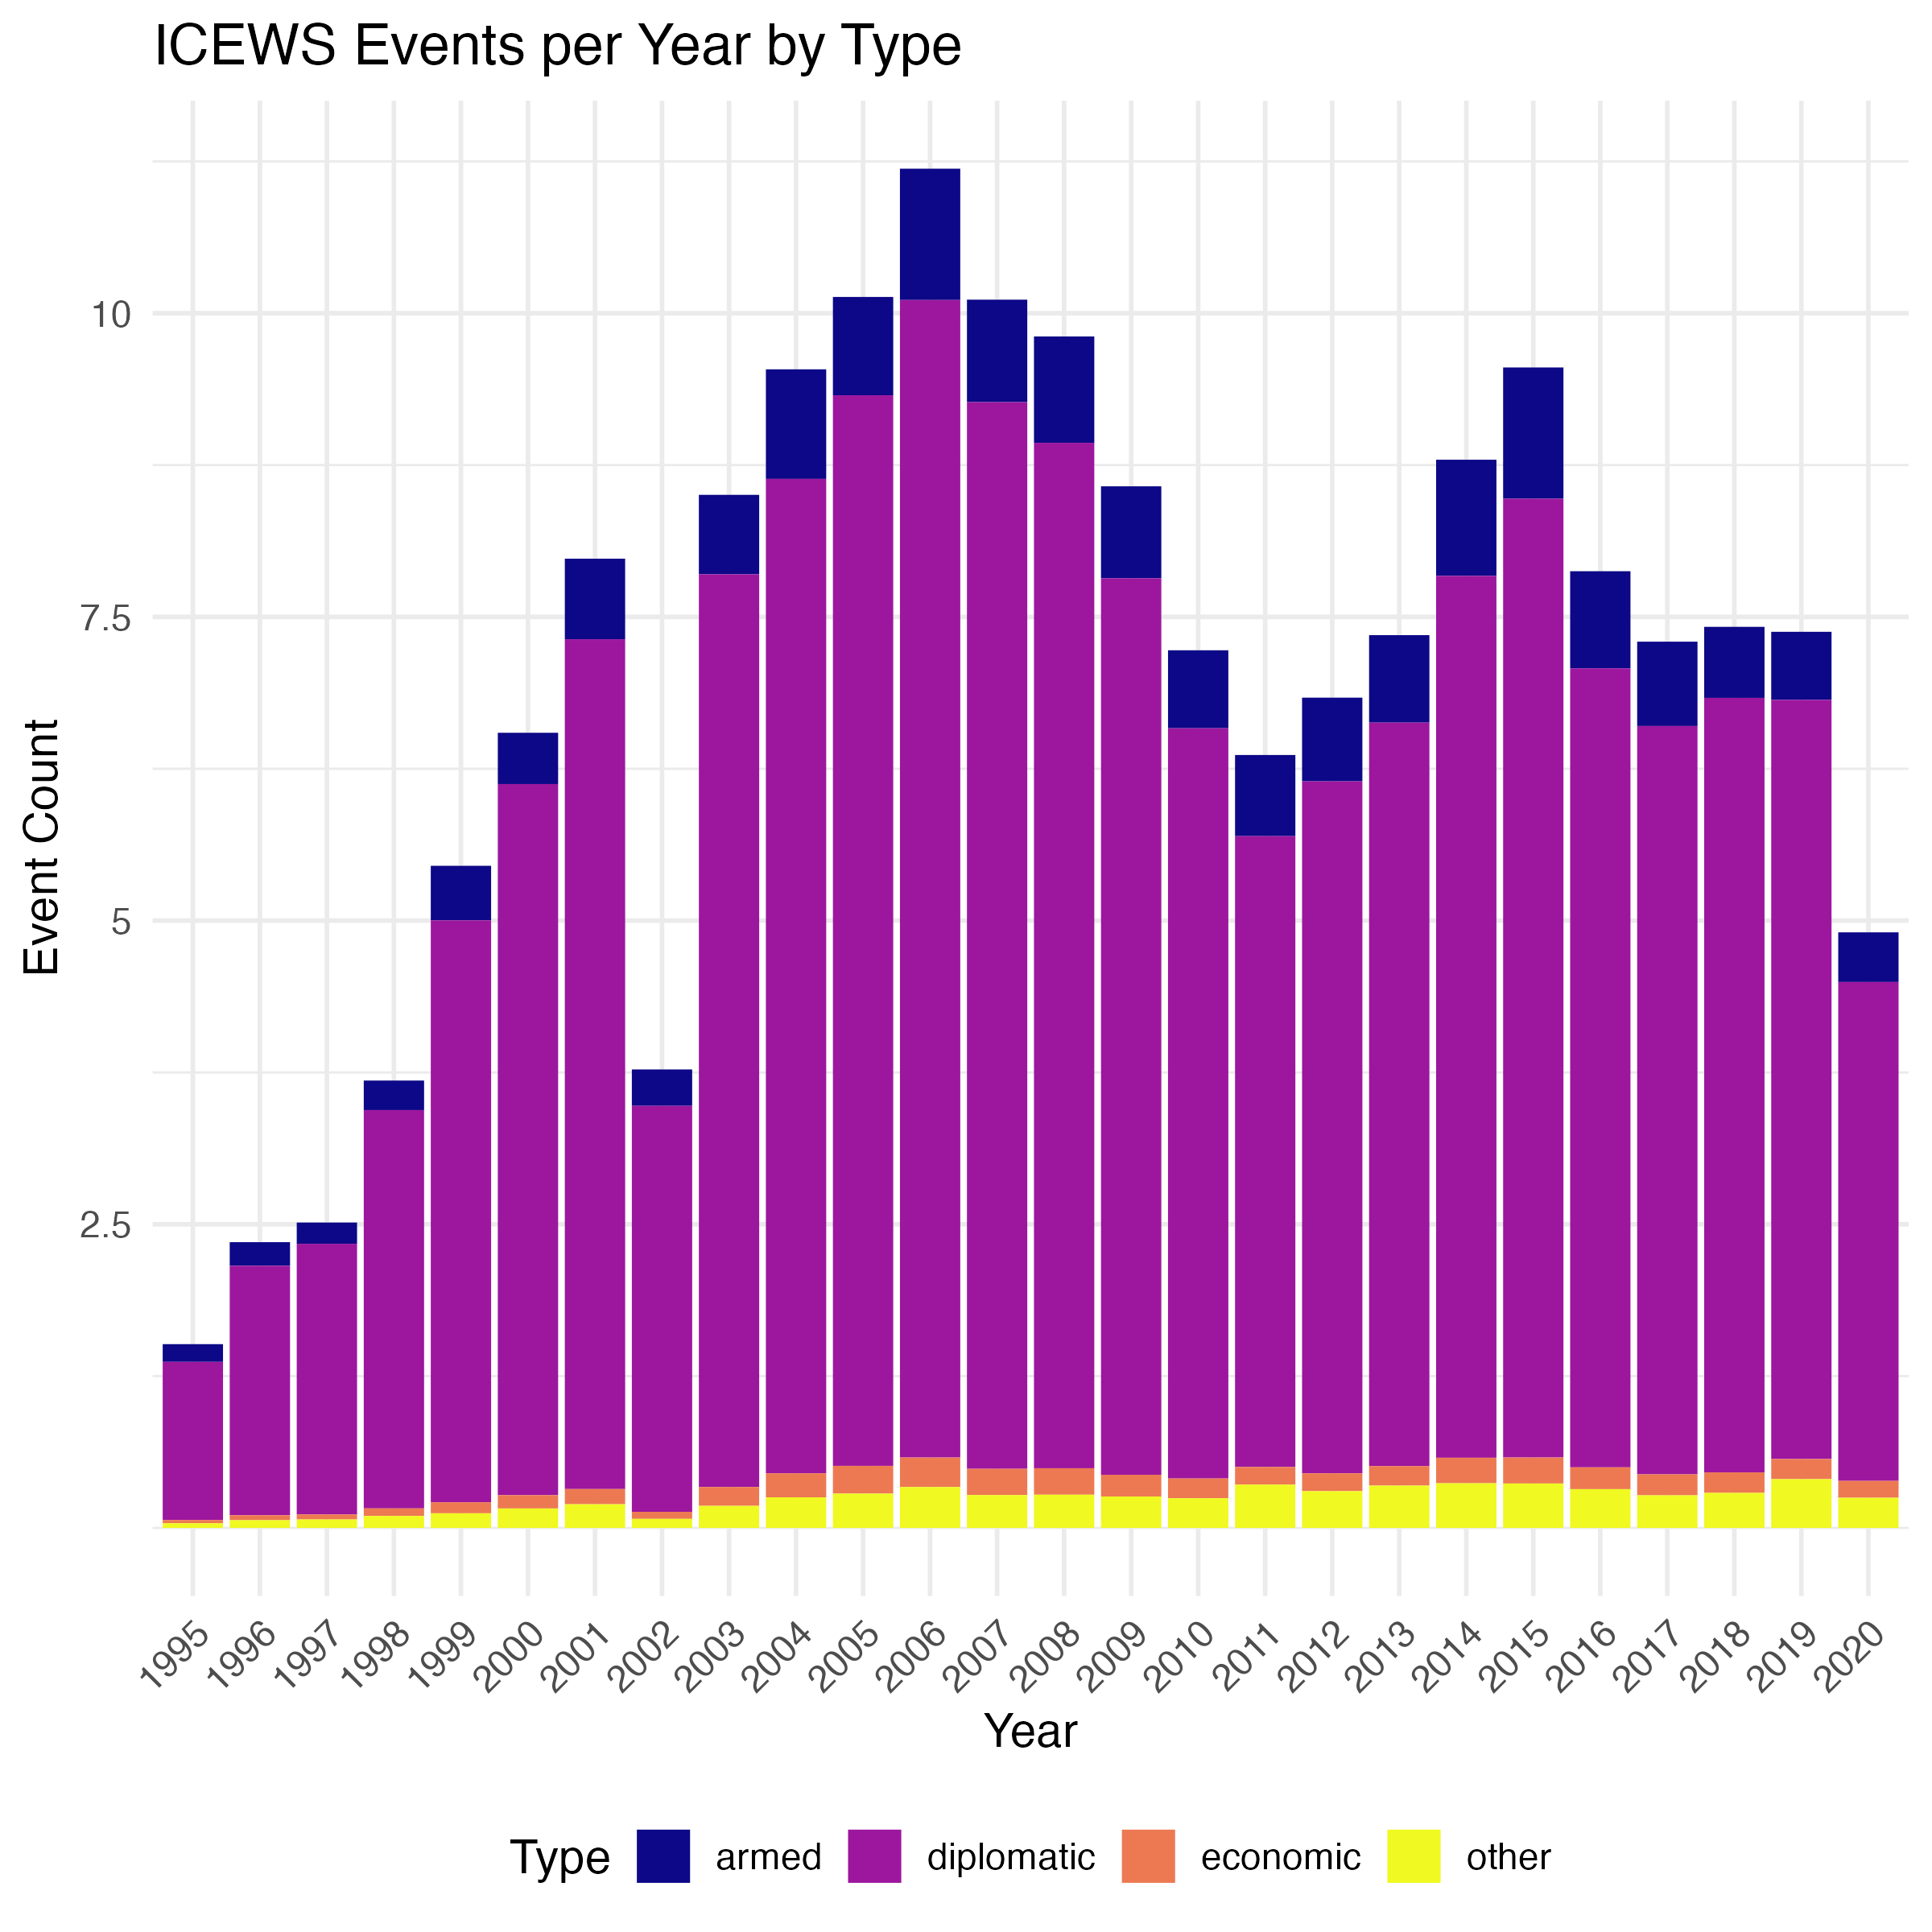
\includegraphics[width=0.8\textwidth]{figures/icews_bar_yearly_stacked.png}
\caption{Monthly Distribution of ICEWS Events by Year}
\end{figure}

By aggregating event-level data into annual averages of Goldstein-scaled intensity scores, the dataset reflects not only the frequency but also the trends of state interactions. This makes ICEWS particularly well-suited for analyzing temporal patterns in international politics. The time series charts below contextualize these trends by visualizing monthly average intensity scores, depicted as points, across three dyads—China, the United States, and Japan—along with short-term (six-month), long-term (twelve-month), and non-parametric (LOESS) smoothers to help interpret underlying shifts in cooperative or conflictual dynamics\footnote{Due to the data constraints, the analysis in the following section uses annual values}. 

An upward trend indicates a growing number and intensity of cooperative actions, while a downward slope reflects the opposite. Focusing on the examples of the United States and China, if the index functions as intended, two patterns should be evident. First, a plateau in relations during the 2000s followed by a visible decline in the mid-2010s, coinciding with the rise of strategic rivalry. Second, sharp dips in the time series should align with major bilateral crises, such as the 1999 U.S. bombing of the Chinese embassy in Belgrade, the 2001 EP-3 spy plane collision, China’s defense budget surge in 2007, the escalation of trade tensions in 2012, and the formal onset of the trade war in 2018. A visual inspection confirms that these inflection points are reflected in the underlying data, lending support to the validity of the intensity-based index.

\clearpage
\begin{landscape}
\begin{figure}[H]
    \centering
    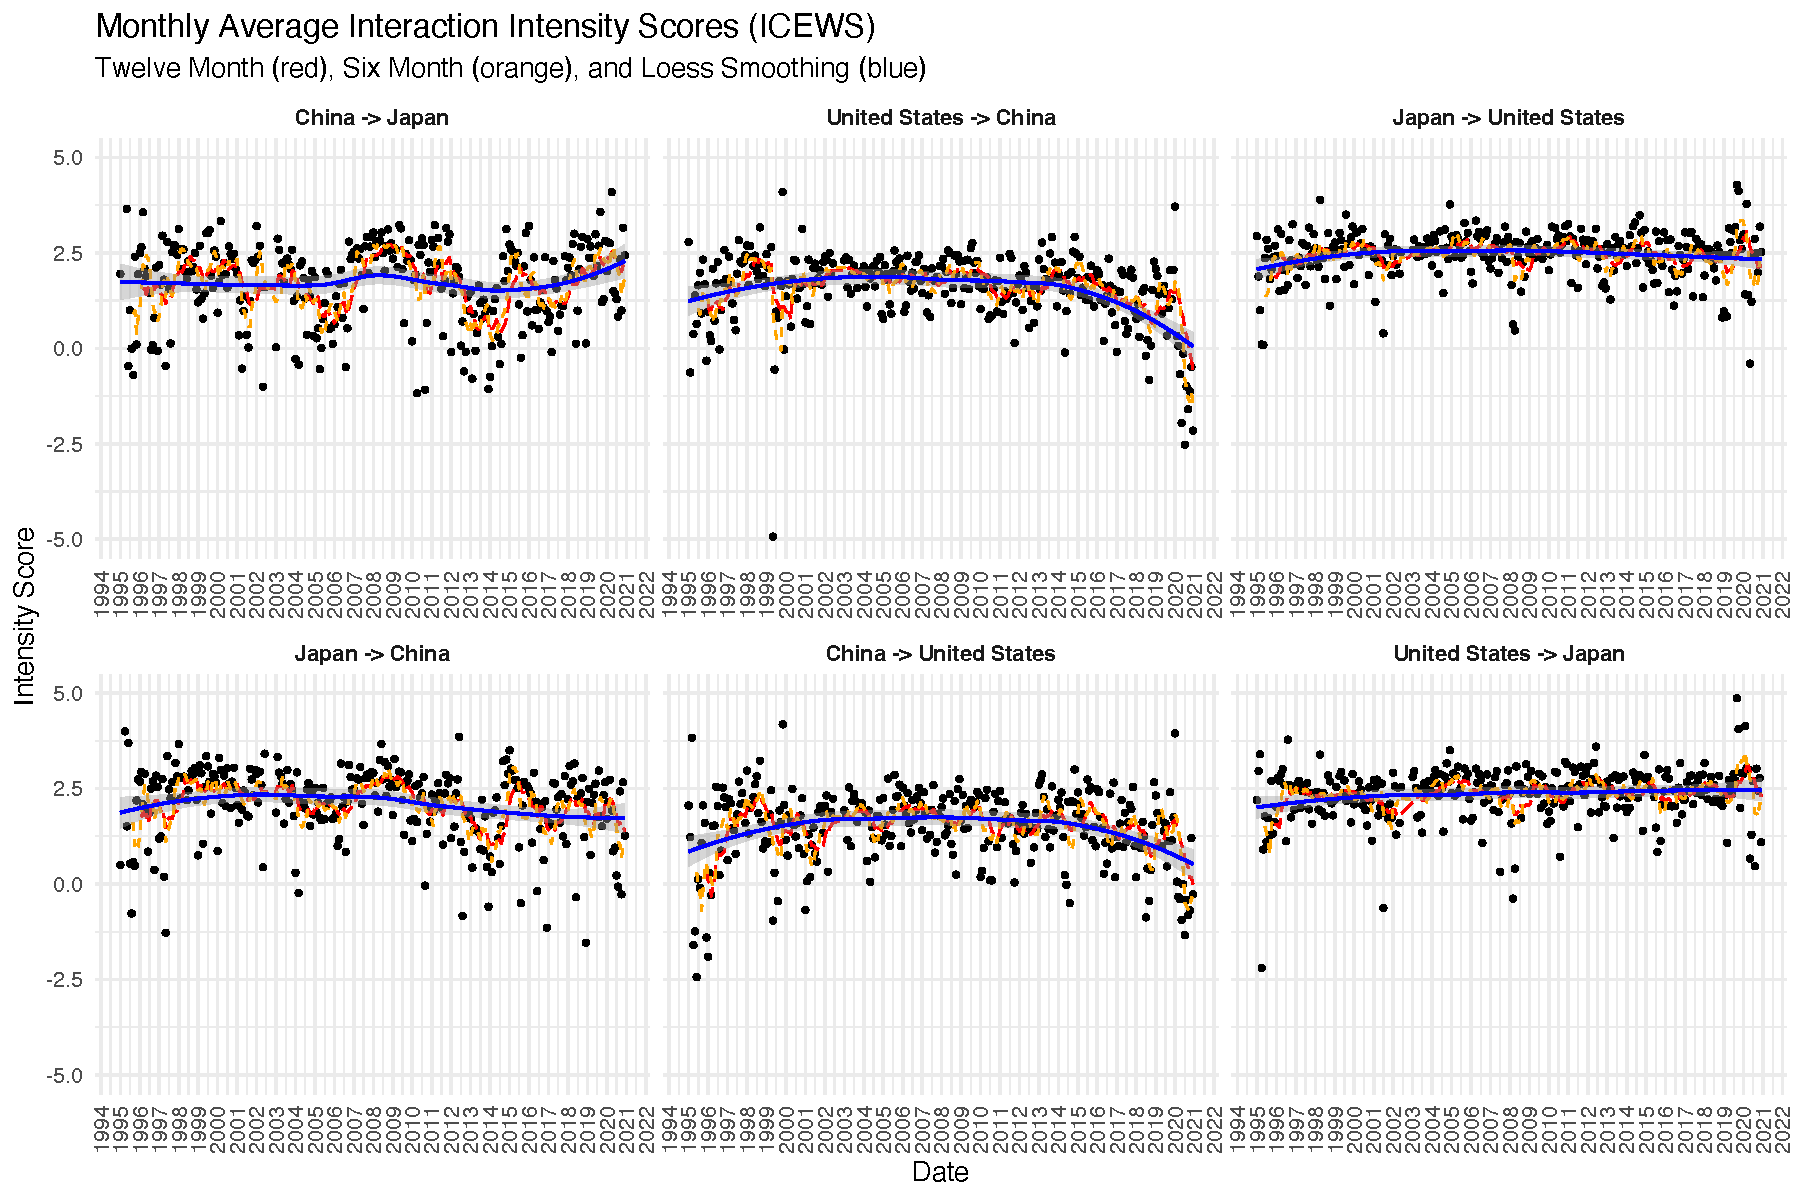
\includegraphics[width=1.4\textwidth]{figures/ICEWS_Directed_Dyads_Faceted.pdf}
    \caption{Monthly Average ICEWS Intensity Scores for Selected Directed Dyads (All Interactions)}
\end{figure}
\end{landscape}
\clearpage

\subsection{Model Specification}
To examine how the composition of trade between countries shapes their political relations, I estimate a series of panel regression models using dyad-year data. The dependent variable in all cases is a continuous measure of bilateral political intensity, constructed from the ICEWS event dataset. For each model, I focus on one of three key structural trade predictors: distance from origin ($D_{ijt}$), cubelet entropy ($H_{ijt}$), or a theory-weighted composite score ($T_{ijt}$). These variables are intended to capture the multidimensional strategic structure of trade between each pair of countries.

To account for unobserved heterogeneity, I estimate ordinary least squares (OLS) models with undirected dyad and year fixed effects. The general form of the model is:
\begin{equation}
Y_{ijt} = \alpha_i + \gamma_t + \beta_k X_{ijt} + \varepsilon_{ijt}
\end{equation}
where $\alpha_i$ and $\gamma_t$ represent undirected dyad and year fixed effects, and $X_{ijt}$ is the focal trade composition variable. This specification ensures that the estimated effects are identified from within-dyad variation over time.

For each compositional measure, the model looks like this:



To assess how the structure of bilateral trade influences political relations between countries, I estimate a series of ordinary least squares (OLS) models using undirected dyad-year panel data. The dependent variable, \( Y_{ijt} \), captures the intensity of political interactions between countries \( i \) and \( j \) in year \( t \), based on event-level data from the Integrated Crisis Early Warning System (ICEWS). Each specification includes a different primary explanatory variable that captures a distinct dimension of trade structure: distance from origin, entropy, or a theory-weighted composite score. All models control for key features of trade interdependence and relative national capabilities, and include dyad and year fixed effects to account for unobserved heterogeneity across country pairs and over time.

The model is specified as follows:

\begin{equation}
\begin{aligned}
Y_{ijt} =\ & \beta_0 + \beta_1 \, \text{MainIV}_{ijt} + \beta_2 \, \text{Salience}_{ijt} + \beta_3 \, \text{Symmetry}_{ijt}
+ \beta_4 \, \text{RegimeDiff}_{ijt} + \beta_5 \, \text{UNDistance}_{ijt} \\
& + \beta_6 \, \text{RelativeGDP}_{ijt} + \beta_7 \, \text{RelativeCINC}_{ijt} + \beta_8 \, \text{RelativeSIPRI}_{ijt}
+ \alpha_i + \gamma_t + \varepsilon_{ijt}
\end{aligned}
\end{equation}

In this equation, the main independent variable, \( \text{MainIV}_{ijt} \), takes one of three forms depending on the specification. When \( \text{MainIV}_{ijt} = \text{Distance}_{ijt} \), the variable measures the average weighted distance of traded goods in the dyad from the global centroid of politically strategic products. When \( \text{MainIV}_{ijt} = \text{Entropy}_{ijt} \), it reflects the entropy of the dyad's trade distribution across cubelets, indicating the level of diversification in traded goods. When \( \text{MainIV}_{ijt} = \text{TheoryWeighted}_{ijt} \), the variable represents a theory-informed composite score that weights trade flows by their hypothesized political salience.

The variable \( \text{Salience}_{ijt} \) denotes the proportion of country \( i \)’s total trade that is conducted with country \( j \), capturing the importance of the bilateral relationship to each actor. \( \text{Symmetry}_{ijt} \) measures the balance of trade flows between the two countries, with higher values indicating greater reciprocity in trade volumes. The control \( \text{RegimeDiff}_{ijt} \) captures the absolute difference in polyarchy scores between the two countries, reflecting variation in political regime types. \( \text{UNDistance}_{ijt} \) measures the ideological distance between countries based on their United Nations voting patterns.

The variables \( \text{RelativeGDP}_{ijt} \), \( \text{RelativeCINC}_{ijt} \), and \( \text{RelativeSIPRI}_{ijt} \) measure the reporter country's size and capabilities relative to its partner in terms of economic output, composite national power, and military spending, respectively. The terms \( \alpha_i \) and \( \gamma_t \) denote dyad and year fixed effects, respectively, while \( \varepsilon_{ijt} \) is the error term. Standard errors are clustered at the dyad level to account for within-dyad correlation over time.

\section{Findings}
\subsection{Overall Interactions}
\rowcolors{2}{gray6}{white}
\begin{table}[htbp]\scriptsize
\centering
\caption{TWFE OLS Coefficients for Mean Intensity, Cooperation, and Conflict}
\renewcommand{\arraystretch}{1.2}
\begin{tabularx}{\textwidth}{
    l
    >{\centering\arraybackslash}X >{\centering\arraybackslash}X >{\centering\arraybackslash}X
    >{\centering\arraybackslash}X >{\centering\arraybackslash}X >{\centering\arraybackslash}X
    >{\centering\arraybackslash}X >{\centering\arraybackslash}X >{\centering\arraybackslash}X
}
\toprule
\rowcolor{gray!20}
 & \multicolumn{3}{c}{\textbf{Mean}} 
 & \multicolumn{3}{c}{\textbf{Cooperation}} 
 & \multicolumn{3}{c}{\textbf{Conflict}} \\
\cmidrule(lr){2-4} \cmidrule(lr){5-7} \cmidrule(lr){8-10}
 & Distance & Entropy & TWS & Distance & Entropy & TWS & Distance & Entropy & TWS \\
\midrule
Distance & $0.022^{}$ (0.018) & -- & -- & $-0.000^{}$ (0.011) & -- & -- & $-0.046^{}$ (0.036) & -- & -- \\
Entropy & -- & $-0.081^{.}$ (0.042) & -- & -- & $-0.016^{}$ (0.024) & -- & -- & $0.076^{}$ (0.081) & -- \\
TWS & -- & -- & $0.029^{*}$ (0.011) & -- & -- & $0.025^{***}$ (0.007) & -- & -- & $0.063^{**}$ (0.025) \\
Salience & $0.115^{}$ (0.167) & $0.074^{}$ (0.166) & $0.131^{}$ (0.165) & $0.153^{*}$ (0.072) & $0.102^{}$ (0.072) & $0.140^{*}$ (0.070) & $0.314^{}$ (0.244) & $0.316^{}$ (0.244) & $0.243^{}$ (0.240) \\
Symmetry & $0.001^{}$ (0.044) & $0.026^{}$ (0.044) & $0.002^{}$ (0.044) & $0.056^{.}$ (0.031) & $0.068^{*}$ (0.031) & $0.057^{.}$ (0.031) & $-0.055^{}$ (0.072) & $-0.055^{}$ (0.074) & $-0.049^{}$ (0.072) \\
Regime Difference & $-0.744^{***}$ (0.138) & $-0.694^{***}$ (0.138) & $-0.746^{***}$ (0.138) & $-0.033^{}$ (0.087) & $-0.005^{}$ (0.087) & $-0.036^{}$ (0.087) & $0.018^{}$ (0.182) & $-0.002^{}$ (0.183) & $0.011^{}$ (0.182) \\
Relative GDP & $0.182^{***}$ (0.050) & $0.196^{***}$ (0.050) & $0.145^{**}$ (0.051) & $0.253^{***}$ (0.019) & $0.254^{***}$ (0.020) & $0.229^{***}$ (0.020) & $0.930^{***}$ (0.096) & $0.916^{***}$ (0.097) & $0.876^{***}$ (0.097) \\
Relative CINC & $-0.203^{***}$ (0.045) & $-0.221^{***}$ (0.046) & $-0.180^{***}$ (0.045) & $-0.171^{***}$ (0.018) & $-0.172^{***}$ (0.019) & $-0.157^{***}$ (0.018) & $-0.561^{***}$ (0.085) & $-0.561^{***}$ (0.086) & $-0.533^{***}$ (0.086) \\
Relative SIPRI & $0.159^{**}$ (0.050) & $0.166^{**}$ (0.051) & $0.156^{**}$ (0.050) & $0.026^{}$ (0.018) & $0.020^{}$ (0.020) & $0.025^{}$ (0.018) & $-0.346^{***}$ (0.100) & $-0.326^{**}$ (0.102) & $-0.340^{***}$ (0.100) \\
UN Distance Score & $-0.082^{*}$ (0.039) & $-0.085^{*}$ (0.039) & $-0.082^{*}$ (0.039) & $-0.019^{}$ (0.026) & $-0.019^{}$ (0.026) & $-0.019^{}$ (0.026) & $0.127^{**}$ (0.049) & $0.126^{*}$ (0.049) & $0.129^{**}$ (0.049) \\
\bottomrule
\end{tabularx}
\begin{tablenotes}
\footnotesize
\item[] \textit{Notes:} Standard errors in parentheses. $^{.} p<0.1$, $^{*} p<0.05$, $^{**} p<0.01$, $^{***} p<0.001$.
\end{tablenotes}
\end{table}

\subsection{Diplomatic Interactions}
\rowcolors{2}{gray6}{white}
\begin{table}[htbp]\scriptsize
\centering
\caption{TWFE OLS Coefficients for Diplomatic Intensity: Mean, Cooperation, and Conflict}
\renewcommand{\arraystretch}{1.2}
\begin{tabularx}{\textwidth}{
  l
  >{\centering\arraybackslash}X >{\centering\arraybackslash}X >{\centering\arraybackslash}X
  >{\centering\arraybackslash}X >{\centering\arraybackslash}X >{\centering\arraybackslash}X
  >{\centering\arraybackslash}X >{\centering\arraybackslash}X >{\centering\arraybackslash}X
}
\toprule
\rowcolor{gray!20}
 & \multicolumn{3}{c}{\textbf{Mean}} 
 & \multicolumn{3}{c}{\textbf{Cooperation}} 
 & \multicolumn{3}{c}{\textbf{Conflict}} \\
\cmidrule(lr){2-4} \cmidrule(lr){5-7} \cmidrule(lr){8-10}
 & Distance & Entropy & TWS & Distance & Entropy & TWS & Distance & Entropy & TWS \\
\midrule
Distance & $0.049^{**}$ (0.016) & -- & -- & $0.010^{}$ (0.010) & -- & -- & $0.039^{}$ (0.026) & -- & -- \\
Entropy & -- & $-0.110^{**}$ (0.035) & -- & -- & $-0.027^{}$ (0.022) & -- & -- & $-0.129^{*}$ (0.059) & -- \\
TWS & -- & -- & $0.009^{}$ (0.009) & -- & -- & $0.012^{.}$ (0.006) & -- & -- & $0.028^{.}$ (0.017) \\
Salience & $0.248^{.}$ (0.132) & $0.234^{.}$ (0.133) & $0.310^{*}$ (0.129) & $0.108^{.}$ (0.065) & $0.068^{}$ (0.065) & $0.115^{.}$ (0.064) & $0.482^{*}$ (0.188) & $0.486^{*}$ (0.189) & $0.508^{**}$ (0.184) \\
Symmetry & $0.059^{}$ (0.038) & $0.069^{.}$ (0.038) & $0.059^{}$ (0.038) & $0.066^{*}$ (0.030) & $0.074^{*}$ (0.031) & $0.066^{*}$ (0.030) & $-0.023^{}$ (0.046) & $-0.024^{}$ (0.047) & $-0.021^{}$ (0.046) \\
Regime Difference & $-0.458^{***}$ (0.112) & $-0.426^{***}$ (0.113) & $-0.460^{***}$ (0.112) & $-0.049^{}$ (0.084) & $-0.036^{}$ (0.085) & $-0.050^{}$ (0.084) & $0.231^{.}$ (0.118) & $0.244^{*}$ (0.119) & $0.227^{.}$ (0.118) \\
Relative GDP & $-0.140^{***}$ (0.038) & $-0.122^{**}$ (0.040) & $-0.165^{***}$ (0.039) & $0.118^{***}$ (0.016) & $0.116^{***}$ (0.017) & $0.103^{***}$ (0.017) & $0.152^{*}$ (0.069) & $0.164^{*}$ (0.070) & $0.112^{}$ (0.071) \\
Relative CINC & $0.036^{}$ (0.036) & $0.026^{}$ (0.038) & $0.055^{}$ (0.037) & $-0.079^{***}$ (0.015) & $-0.078^{***}$ (0.016) & $-0.069^{***}$ (0.015) & $-0.116^{.}$ (0.063) & $-0.124^{.}$ (0.064) & $-0.087^{}$ (0.064) \\
Relative SIPRI & $0.154^{***}$ (0.037) & $0.147^{***}$ (0.039) & $0.148^{***}$ (0.037) & $-0.014^{}$ (0.016) & $-0.019^{}$ (0.017) & $-0.016^{}$ (0.016) & $-0.064^{}$ (0.067) & $-0.057^{}$ (0.069) & $-0.070^{}$ (0.067) \\
UN Distance Score & $-0.082^{*}$ (0.033) & $-0.087^{**}$ (0.033) & $-0.082^{*}$ (0.032) & $-0.018^{}$ (0.025) & $-0.016^{}$ (0.025) & $-0.018^{}$ (0.025) & $0.050^{}$ (0.035) & $0.048^{}$ (0.035) & $0.050^{}$ (0.035) \\
\bottomrule
\end{tabularx}
\begin{tablenotes}
\footnotesize
\item[] \textit{Notes:} Standard errors in parentheses. $^{.} p<0.1$, $^{*} p<0.05$, $^{**} p<0.01$, $^{***} p<0.001$.}
\end{tablenotes}
\end{table}

\subsection{Armed Interactions}
\rowcolors{2}{gray6}{white}
\begin{table}[htbp]\scriptsize
\centering
\caption{TWFE OLS Coefficients for Armed Intensity: Mean, Cooperation, and Conflict}
\renewcommand{\arraystretch}{1.2}
\begin{tabularx}{\textwidth}{
  l
  >{\centering\arraybackslash}X >{\centering\arraybackslash}X >{\centering\arraybackslash}X
  >{\centering\arraybackslash}X >{\centering\arraybackslash}X >{\centering\arraybackslash}X
  >{\centering\arraybackslash}X >{\centering\arraybackslash}X >{\centering\arraybackslash}X
}
\toprule
\rowcolor{gray!20}
 & \multicolumn{3}{c}{\textbf{Mean}} 
 & \multicolumn{3}{c}{\textbf{Cooperation}} 
 & \multicolumn{3}{c}{\textbf{Conflict}} \\
\cmidrule(lr){2-4} \cmidrule(lr){5-7} \cmidrule(lr){8-10}
 & Distance & Entropy & TWS & Distance & Entropy & TWS & Distance & Entropy & TWS \\
\midrule
Distance & $-0.427^{*}$ (0.189) & -- & -- & $0.062^{}$ (0.050) & -- & -- & $0.048^{}$ (0.030) & -- & -- \\
Entropy & -- & $0.779^{.}$ (0.453) & -- & -- & $-0.166^{}$ (0.114) & -- & -- & $-0.076^{}$ (0.068) & -- \\
TWS & -- & -- & $0.117^{}$ (0.103) & -- & -- & $-0.020^{}$ (0.031) & -- & -- & $-0.023^{}$ (0.020) \\
Salience & $1.819^{.}$ (1.009) & $1.526^{}$ (1.023) & $1.424^{}$ (1.015) & $0.250^{}$ (0.461) & $0.328^{}$ (0.463) & $0.297^{}$ (0.453) & $0.263^{}$ (0.191) & $0.222^{}$ (0.194) & $0.308^{.}$ (0.186) \\
Symmetry & $-0.749^{*}$ (0.357) & $-0.591^{}$ (0.368) & $-0.730^{*}$ (0.358) & $-0.155^{}$ (0.109) & $-0.173^{}$ (0.113) & $-0.156^{}$ (0.109) & $0.014^{}$ (0.058) & $0.024^{}$ (0.060) & $0.010^{}$ (0.058) \\
Regime Difference & $-2.286^{*}$ (0.923) & $-2.315^{*}$ (0.933) & $-2.342^{*}$ (0.921) & $0.064^{}$ (0.291) & $0.076^{}$ (0.293) & $0.078^{}$ (0.290) & $0.168^{}$ (0.154) & $0.176^{}$ (0.156) & $0.174^{}$ (0.154) \\
Relative GDP & $3.238^{***}$ (0.445) & $3.074^{***}$ (0.452) & $3.231^{***}$ (0.450) & $-0.328^{*}$ (0.129) & $-0.293^{*}$ (0.132) & $-0.334^{*}$ (0.133) & $0.320^{***}$ (0.077) & $0.284^{***}$ (0.079) & $0.333^{***}$ (0.079) \\
Relative CINC & $-1.566^{***}$ (0.383) & $-1.501^{***}$ (0.388) & $-1.594^{***}$ (0.385) & $-0.103^{}$ (0.100) & $-0.118^{}$ (0.099) & $-0.093^{}$ (0.100) & $0.014^{}$ (0.063) & $0.051^{}$ (0.062) & $0.009^{}$ (0.063) \\
Relative SIPRI & $-0.807^{.}$ (0.445) & $-0.793^{.}$ (0.456) & $-0.770^{.}$ (0.442) & $0.400^{***}$ (0.115) & $0.412^{***}$ (0.116) & $0.398^{***}$ (0.115) & $-0.190^{**}$ (0.073) & $-0.200^{**}$ (0.074) & $-0.195^{**}$ (0.073) \\
UN Distance Score & $-0.283^{}$ (0.273) & $-0.234^{}$ (0.276) & $-0.279^{}$ (0.273) & $0.038^{}$ (0.090) & $0.036^{}$ (0.091) & $0.038^{}$ (0.090) & $0.037^{}$ (0.041) & $0.044^{}$ (0.042) & $0.037^{}$ (0.041) \\
\bottomrule
\end{tabularx}
\begin{tablenotes}
\footnotesize
\item[] \textit{Notes:} Standard errors in parentheses. $^{.} p<0.1$, $^{*} p<0.05$, $^{**} p<0.01$, $^{***} p<0.001$.}
\end{tablenotes}
\end{table}

\subsection{Economic Interactions}
\rowcolors{2}{gray6}{white}
\begin{table}[htbp]\scriptsize
\centering
\caption{TWFE OLS Coefficients for Economic Intensity: Mean, Cooperation, and Conflict}
\renewcommand{\arraystretch}{1.2}
\begin{tabularx}{\textwidth}{
  l
  >{\centering\arraybackslash}X >{\centering\arraybackslash}X >{\centering\arraybackslash}X
  >{\centering\arraybackslash}X >{\centering\arraybackslash}X >{\centering\arraybackslash}X
  >{\centering\arraybackslash}X >{\centering\arraybackslash}X >{\centering\arraybackslash}X
}
\toprule
\rowcolor{gray!20}
 & \multicolumn{3}{c}{\textbf{Mean}} 
 & \multicolumn{3}{c}{\textbf{Cooperation}} 
 & \multicolumn{3}{c}{\textbf{Conflict}} \\
\cmidrule(lr){2-4} \cmidrule(lr){5-7} \cmidrule(lr){8-10}
 & Distance & Entropy & TWS & Distance & Entropy & TWS & Distance & Entropy & TWS \\
\midrule
Distance & $-0.034^{}$ (0.120) & -- & -- & $-0.093^{**}$ (0.034) & -- & -- & $0.334^{*}$ (0.146) & -- & -- \\
Entropy & -- & $0.090^{}$ (0.284) & -- & -- & $0.198^{*}$ (0.080) & -- & -- & $-0.891^{**}$ (0.315) & -- \\
TWS & -- & -- & $0.176^{*}$ (0.078) & -- & -- & $0.086^{***}$ (0.022) & -- & -- & $-0.017^{}$ (0.135) \\
Salience & $0.082^{}$ (0.756) & $0.134^{}$ (0.756) & $-0.039^{}$ (0.729) & $0.235^{}$ (0.194) & $0.200^{}$ (0.192) & $0.112^{}$ (0.194) & $-2.261^{**}$ (0.790) & $-2.287^{**}$ (0.791) & $-1.984^{*}$ (0.833) \\
Symmetry & $0.050^{}$ (0.209) & $0.074^{}$ (0.211) & $0.063^{}$ (0.209) & $-0.072^{}$ (0.058) & $-0.072^{}$ (0.058) & $-0.067^{}$ (0.057) & $0.124^{}$ (0.236) & $0.067^{}$ (0.239) & $0.080^{}$ (0.234) \\
Regime Difference & $-2.772^{***}$ (0.525) & $-2.790^{***}$ (0.528) & $-2.790^{***}$ (0.524) & $-0.186^{}$ (0.133) & $-0.180^{}$ (0.133) & $-0.196^{}$ (0.132) & $0.158^{}$ (0.636) & $0.146^{}$ (0.636) & $0.154^{}$ (0.634) \\
Relative GDP & $0.657^{*}$ (0.302) & $0.653^{*}$ (0.302) & $0.479^{}$ (0.298) & $0.888^{***}$ (0.081) & $0.888^{***}$ (0.082) & $0.835^{***}$ (0.084) & $-0.841^{*}$ (0.369) & $-0.801^{*}$ (0.371) & $-0.932^{*}$ (0.416) \\
Relative CINC & $-0.674^{**}$ (0.257) & $-0.703^{**}$ (0.259) & $-0.578^{*}$ (0.260) & $-0.517^{***}$ (0.071) & $-0.517^{***}$ (0.071) & $-0.493^{***}$ (0.072) & $0.435^{}$ (0.334) & $0.469^{}$ (0.335) & $0.559^{.}$ (0.330) \\
Relative SIPRI & $0.760^{**}$ (0.285) & $0.796^{**}$ (0.287) & $0.766^{**}$ (0.285) & $0.107^{}$ (0.073) & $0.093^{}$ (0.075) & $0.111^{}$ (0.073) & $-0.331^{}$ (0.351) & $-0.349^{}$ (0.355) & $-0.355^{}$ (0.353) \\
UN Distance Score & $-0.255^{}$ (0.161) & $-0.250^{}$ (0.163) & $-0.253^{}$ (0.162) & $0.026^{}$ (0.041) & $0.031^{}$ (0.041) & $0.026^{}$ (0.041) & $0.135^{}$ (0.177) & $0.128^{}$ (0.179) & $0.125^{}$ (0.178) \\
\bottomrule
\end{tabularx}
\begin{tablenotes}
\footnotesize
\item[] \textit{Notes:} Standard errors in parentheses. $^{.} p<0.1$, $^{*} p<0.05$, $^{**} p<0.01$, $^{***} p<0.001$.}
\end{tablenotes}
\end{table}

\subsection{Alternative Explanations}
\rowcolors{2}{gray6}{white}
\begin{table}[htbp]
\scriptsize
\centering
\caption{Regression Results: Trade Variables Lagged and Lead by 1 Year}
\renewcommand{\arraystretch}{1.2}
\begin{tabularx}{\textwidth}{l
  >{\centering\arraybackslash}X
  >{\centering\arraybackslash}X
  >{\centering\arraybackslash}X
  >{\centering\arraybackslash}X
  >{\centering\arraybackslash}X
  >{\centering\arraybackslash}X}
\toprule
\rowcolor{gray!20}
& \multicolumn{3}{c}{Lagged (t$-$1)} & \multicolumn{3}{c}{Lead (t$+$1)} \\
\cmidrule(lr){2-4} \cmidrule(lr){5-7}
Variable & Distance & Entropy & TWS & Distance & Entropy & TWS \\
\midrule
Distance                & $-0.017^{}$ (0.018) & --                  & --                  & $0.004^{}$ (0.018)  & --                  & --                  \\
Entropy                 & --                  & $-0.003^{}$ (0.041) & --                  & --                  & $-0.033^{}$ (0.039) & --                  \\
Theory-weighted Share   & --                  & --                  & $-0.027^{*}$ (0.011) & --                  & --                  & $-0.039^{***}$ (0.011) \\
Salience                & $0.103^{}$ (0.169)  & $0.091^{}$ (0.168)  & $0.115^{}$ (0.168)  & $0.149^{}$ (0.166)  & $0.145^{}$ (0.164)  & $0.141^{}$ (0.164)  \\
Symmetry                & $-0.003^{}$ (0.044) & $-0.000^{}$ (0.045) & $-0.004^{}$ (0.044) & $0.002^{}$ (0.044)  & $0.017^{}$ (0.045)  & $-0.001^{}$ (0.044) \\
Regime Diff. (Polyarchy)& $-0.702^{***}$ (0.140) & $-0.687^{***}$ (0.141) & $-0.696^{***}$ (0.140) & $-0.740^{***}$ (0.138) & $-0.730^{***}$ (0.138) & $-0.733^{***}$ (0.138) \\
UN Distance Score       & $-0.070^{.}$ (0.039) & $-0.072^{.}$ (0.039) & $-0.070^{.}$ (0.039) & $-0.084^{*}$ (0.038) & $-0.081^{*}$ (0.039) & $-0.084^{*}$ (0.038) \\
Relative GDP            & $0.184^{***}$ (0.050) & $0.170^{***}$ (0.050) & $0.156^{**}$ (0.051) & $0.175^{***}$ (0.049) & $0.168^{***}$ (0.050) & $0.143^{**}$ (0.050) \\
Relative CINC           & $-0.211^{***}$ (0.046) & $-0.199^{***}$ (0.047) & $-0.193^{***}$ (0.046) & $-0.196^{***}$ (0.045) & $-0.210^{***}$ (0.046) & $-0.177^{***}$ (0.045) \\
Relative SIPRI          & $0.159^{**}$ (0.050) & $0.154^{**}$ (0.050) & $0.157^{**}$ (0.050) & $0.154^{**}$ (0.050) & $0.169^{***}$ (0.050) & $0.154^{**}$ (0.050) \\
\bottomrule
\end{tabularx}
\begin{tablenotes}
\footnotesize
\item[] \textit{Notes:} Standard errors in parentheses. TWS = Theory-weighted Share. $^{*} p<0.05$, $^{**} p<0.01$, $^{***} p<0.001$, $^{.} p<0.1$.
\end{tablenotes}
\end{table}

\section{Implications}

\clearpage

\printbibliography

\clearpage

\section{Appendix}
\subsection{Trade Data}
\begin{table}[htbp]
\centering
\caption{Cubelet Share Composition by Directed Dyad (2020)}
\begin{tabularx}{\textwidth}{ll*{8}{>{\centering\arraybackslash}X}}
\toprule
Exporter & Importer & HHL & HLH & HLL & LHL & LLL & HHH & LHH & LLH \\
\midrule
CHN & USA & 0.32 & 0.24 & 0.08 & 0.03 & 0.01 & 0.28 & 0.02 & 0.01 \\
CHN & JPN & 0.29 & 0.26 & 0.15 & 0.04 & 0.02 & 0.20 & 0.03 & 0.01 \\
USA & CHN & 0.26 & 0.42 & 0.17 & 0.02 & 0.00 & 0.09 & 0.03 & 0.02 \\
USA & JPN & 0.24 & 0.38 & 0.17 & 0.02 & 0.01 & 0.15 & 0.02 & 0.01 \\
JPN & USA & 0.03 & 0.77 & 0.05 & 0.01 & 0.00 & 0.11 & 0.02 & 0.02 \\
JPN & CHN & 0.03 & 0.60 & 0.10 & 0.01 & 0.01 & 0.19 & 0.04 & 0.03 \\
\bottomrule
\end{tabularx}
\end{table}

\subsection{ICEWS Data}
The heatmap below displays monthly event counts across years to visualize the temporal completeness of the ICEWS data and identify periods of irregular coverage. The data has extensive coverage following 2000, with the exception of 2002.

\begin{figure}[H]
\centering
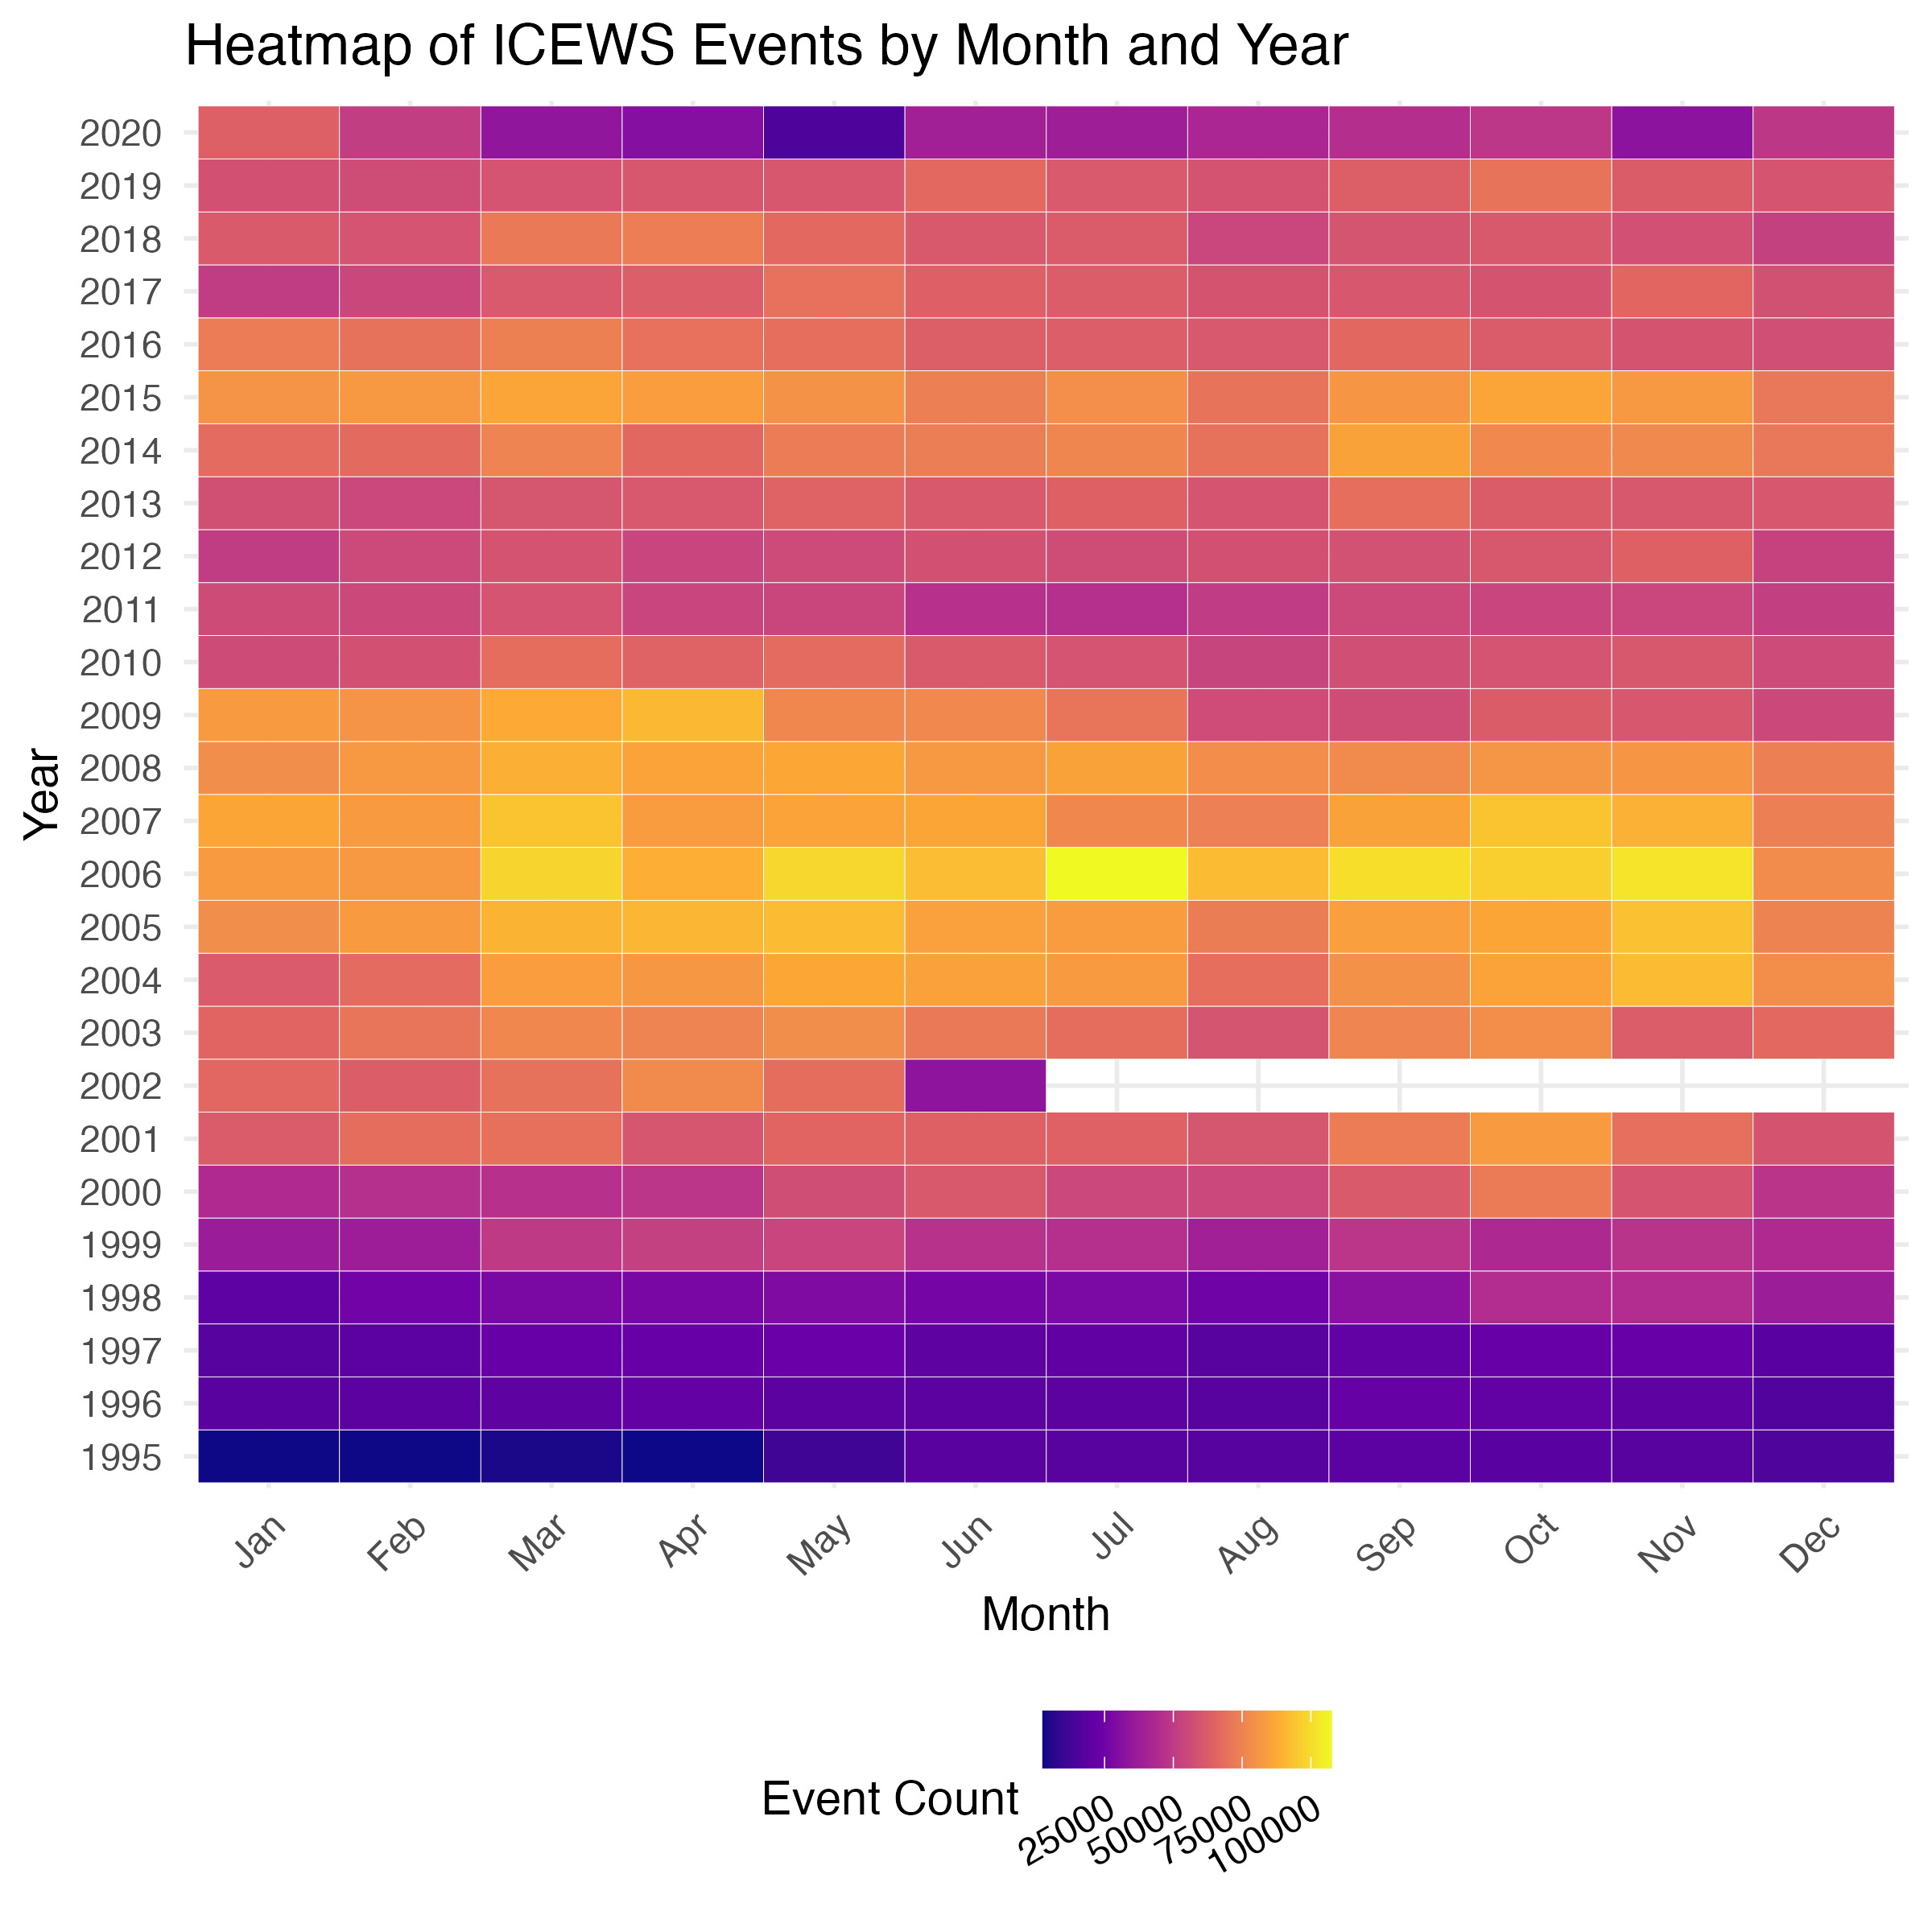
\includegraphics[width=0.9\textwidth]{figures/icews_heatmap_monthly.png}
\caption{Annual ICEWS Events by Type (in 100,000s)}
\end{figure}

The ridge density plots below visualize the distribution of Goldstein-scale intensity scores over time. Values to the left of 0 mark instances of conflict, and to right, instances of cooperation. Values farther away from 0 indicate higher intensity interactions. The figure below reveals a consistently modal distribution centered around 0, with long tails. 

\begin{figure}[H]
\centering
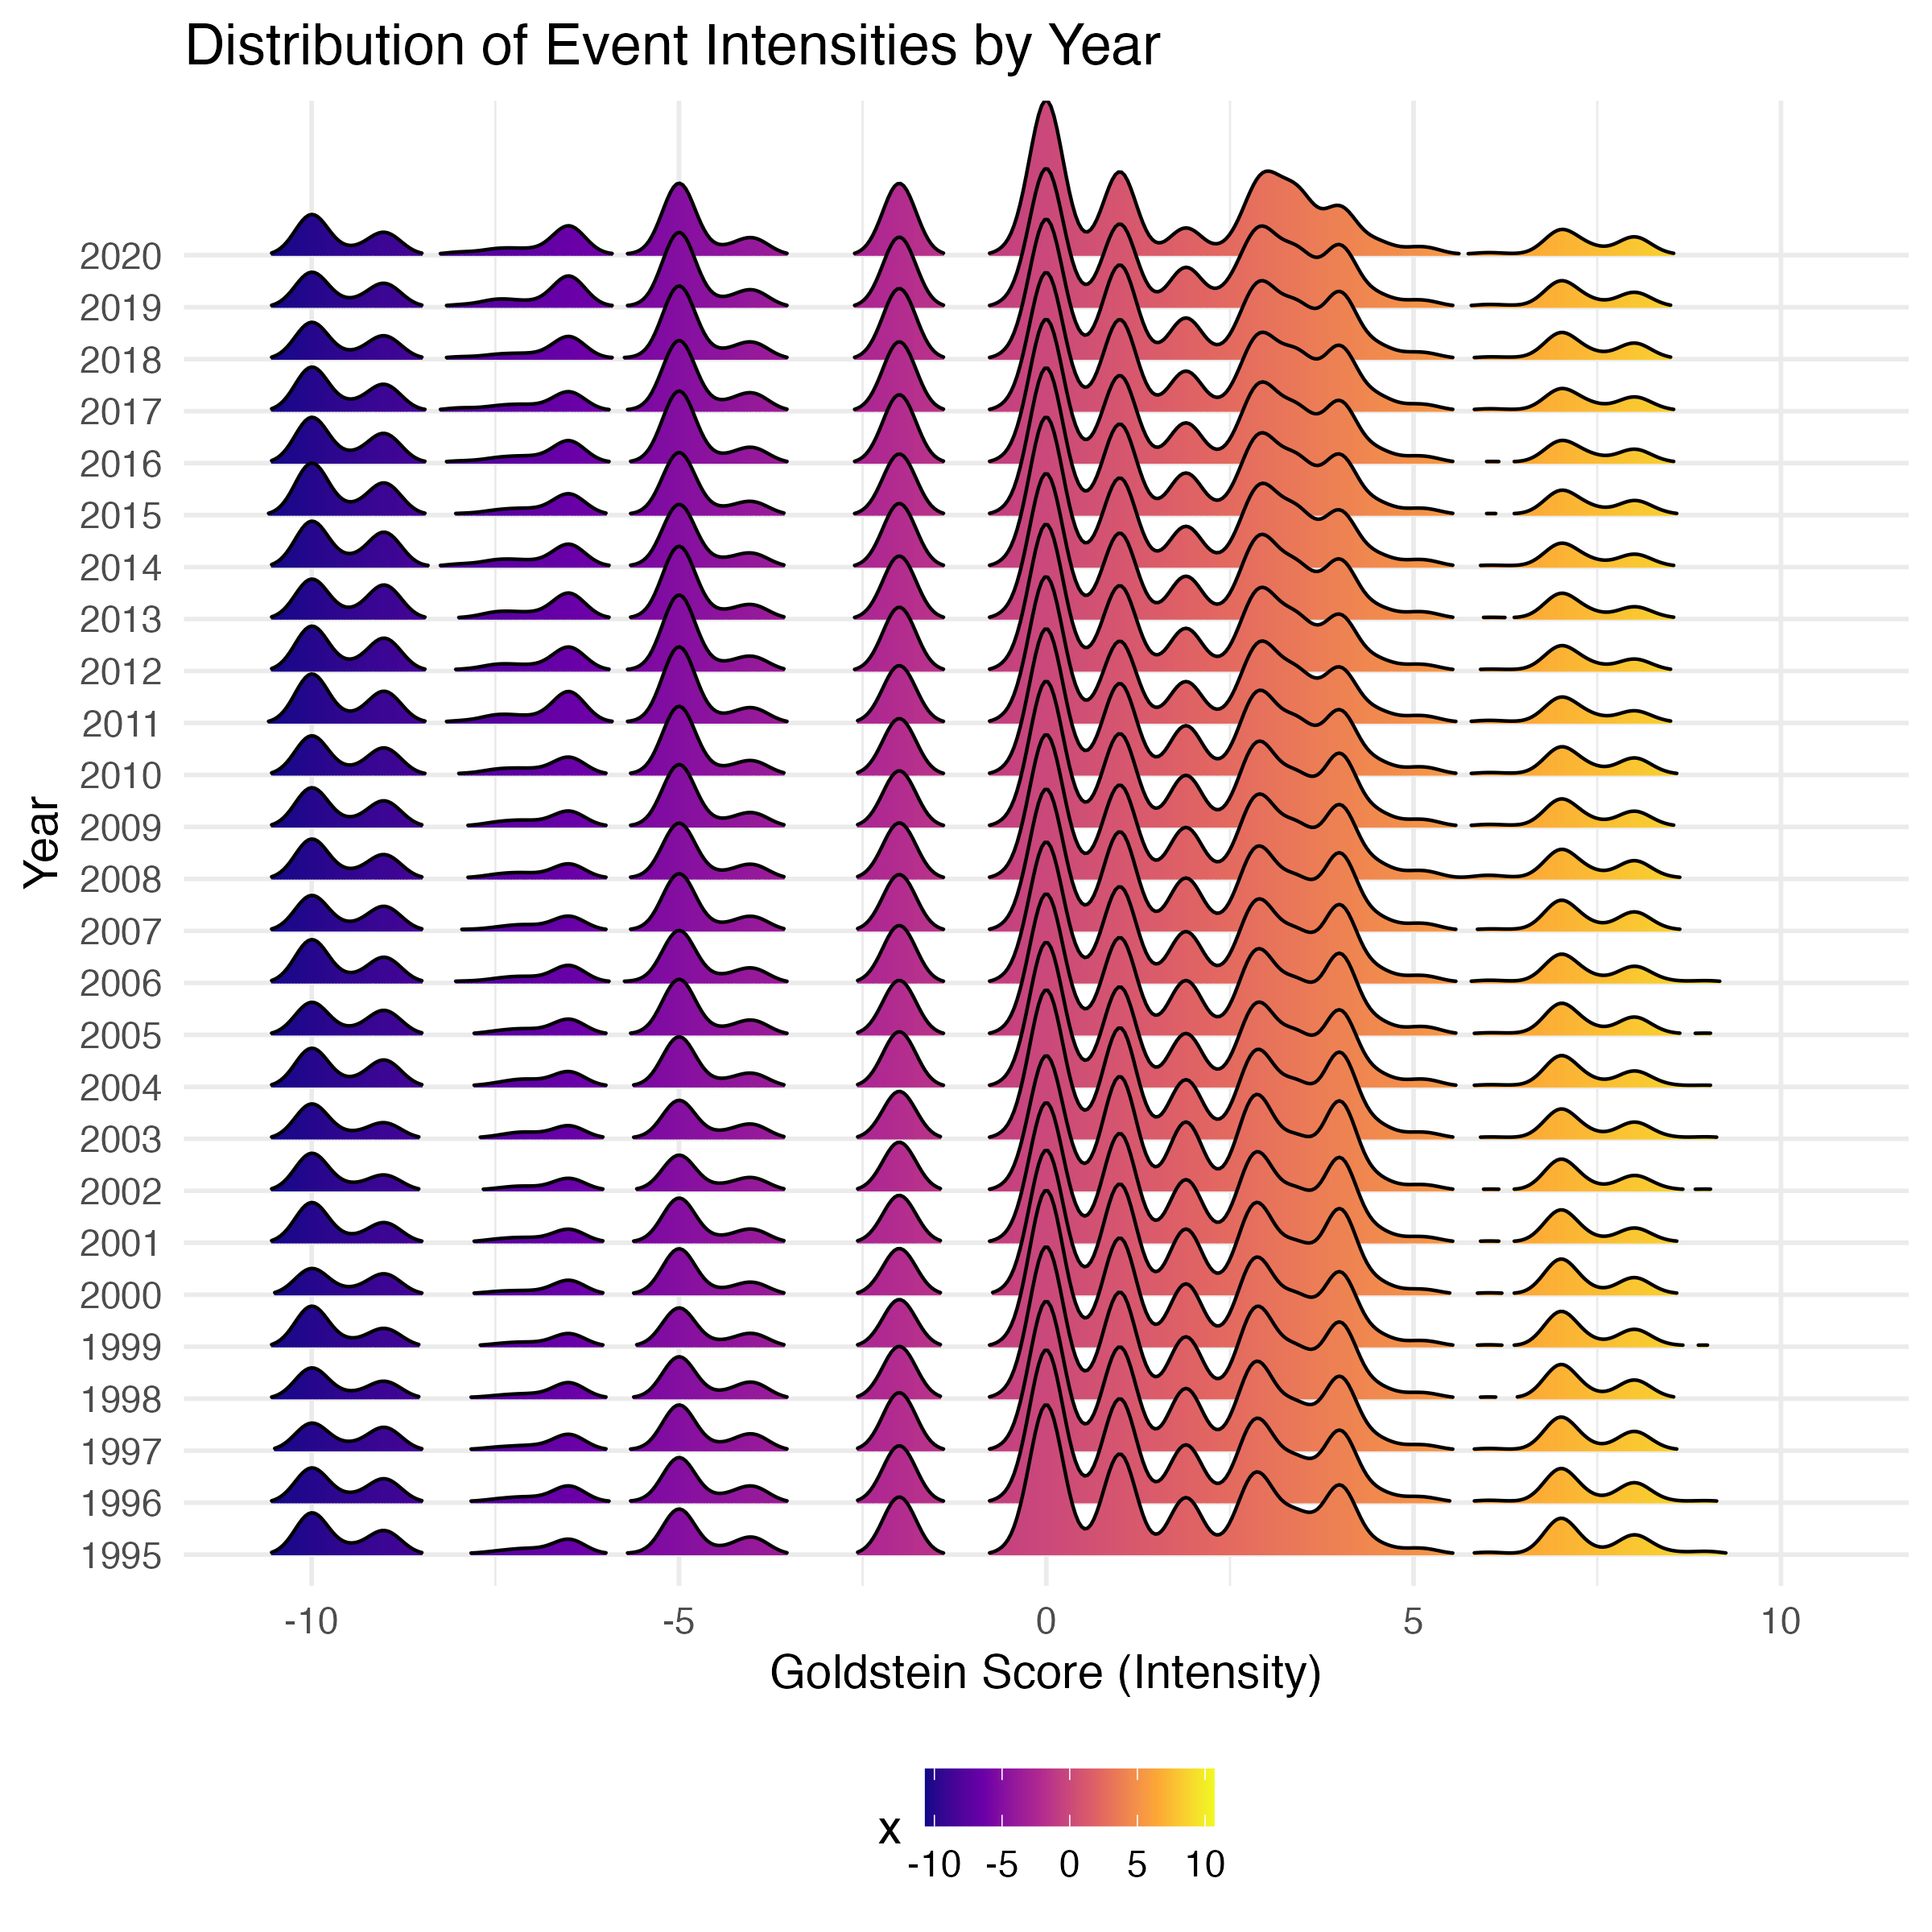
\includegraphics[width=0.8\textwidth]{figures/icews_ridge_intensity_by_year.png}
\caption{Density of Event Intensities by Year}
\end{figure}
\subsection{Summary Statistics}
Table below provides summary statistics for the variables.
\rowcolors{2}{gray!10}{white}
\begin{table}[htbp]
\scriptsize
\centering
\caption{Descriptive Statistics for Regression Variables}
\renewcommand{\arraystretch}{1.2}
\begin{tabularx}{\textwidth}{lXrrrrr}
\toprule
\rowcolor{gray!20}
Group & Variable & \textbf{N} & \textbf{Mean} & \textbf{SD} & \textbf{Min} & \textbf{Max} \\
\midrule
Dependent Variables
 & Overall Mean & 170598 & 1.978 & 2.366 & -10 & 10 \\
 & Overall Mean: Cooperation & 157791 & 3.194 & 1.392 & 0.4 & 10 \\
 & Overall Mean: Conflict & 64769 & -4.63 & 2.194 & -10 & -0.1 \\
 & Diplomatic Mean & 167374 & 2.123 & 1.948 & -9.5 & 9 \\
 & Diplomatic Mean: Cooperation & 155515 & 3.057 & 1.308 & 0.4 & 9 \\
 & Diplomatic Mean: Conflict & 56985 & -3.515 & 1.362 & -9.5 & -0.1 \\
 & Armed Mean & 26865 & -4.22 & 6.871 & -10 & 10 \\
 & Armed Mean: Cooperation & 11493 & 7.352 & 1.353 & 3.4 & 10 \\
 & Armed Mean: Conflict & 21264 & -9.075 & 0.974 & -10 & -4 \\
 & Economic Mean: Intensity & 30219 & 4.316 & 4.11 & -9.2 & 7.4 \\
 & Economic Mean: Intensity: Cooperation & 27712 & 6.034 & 1.023 & 3.4 & 7.4 \\
 & Economic Mean: Intensity: Conflict & 6243 & -6.937 & 1.943 & -9.2 & -0.3 \\
Independent Variables
 & Distance & 389630 & 1.564 & 0.479 & 0.028 & 2.887 \\
 & Entropy & 338387 & 0.542 & 0.239 & 0 & 1 \\
 & Theory-weighted Share & 389630 & -0.007 & 0.979 & -3.855 & 2.108 \\
 & Salience & 389630 & 0.009 & 0.038 & 0 & 0.992 \\
 & Symmetry & 389630 & 0.284 & 0.302 & 0 & 1 \\
Controls
 & Both NATO & 386295 & 0.012 & 0.11 & 0 & 1 \\
 & Both WTO & 386295 & 0.261 & 0.439 & 0 & 1 \\
 & Regime Diff. (Polyarchy) & 354115 & 0.308 & 0.223 & 0 & 0.909 \\
 & Relative CINC & 311250 & 0.55 & 0.362 & 0 & 1 \\
 & Relative GDP & 381573 & 0.567 & 0.379 & 0 & 1 \\
 & Relative SIPRI & 310938 & 0.542 & 0.389 & 0 & 1 \\
 & UN Distance Score & 383765 & 1.019 & 0.788 & 0 & 4.818 \\
\bottomrule
\end{tabularx}
\begin{tablenotes}
\footnotesize
\item[] \textit{Notes:} Variables shown are used in regression specifications below.
\end{tablenotes}
\end{table}


\end{document}
